%%% ======= Beamer ======
\documentclass[usenames,dvipsnames,t]{beamer}
% \documentclass[usenames,dvipsnames, handout]{beamer}
\beamertemplatenavigationsymbolsempty % remove toolbar at the bottom of slides
\usepackage{appendixnumberbeamer} % for appendix
\usetheme{Madrid}
\usecolortheme{default}
\useinnertheme{circles}

\usepackage{fontawesome}
\usepackage{colortbl}  % For \cellcolor in tables


% Define commands for social media icons with links
\newcommand{\linkedin}{\href{https://www.linkedin.com/in/ThibeauWouters}{\textcolor{black}{\faLinkedin}}}
\newcommand{\github}{\href{https://github.com/ThibeauWouters}{\textcolor{black}{\faGithub}}}
\newcommand{\myemail}{\href{mailto:t.r.i.wouters@uu.nl}{\textcolor{black}{\faEnvelope}}}

\newcommand{\ghlink}[1]{\href{https://github.com/#1}{\textcolor{black}{\faGithub}}}

\definecolor{customblue}{HTML}{7db8dc}
\newcommand{\thetaeos}{\boldsymbol{\theta}_{\rm{EOS}}}
\newcommand{\boldtheta}{\boldsymbol{\theta}}

\setbeamercolor{author in head/foot}{bg=blue!10, fg=blue}
\setbeamercolor{title in head/foot}{bg=blue!10, fg=blue}
\setbeamercolor{date in head/foot}{bg=blue!10, fg=blue}

\makeatletter
\setbeamertemplate{footline}{
  \leavevmode%
  \hbox{%
  \begin{beamercolorbox}[wd=.333333\paperwidth,ht=2.25ex,dp=1ex,center]{author in head/foot}%
    \usebeamerfont{author in head/foot}\insertshortauthor\expandafter\ifblank\expandafter{\beamer@shortinstitute}{}{~~(\insertshortinstitute)}
  \end{beamercolorbox}%
  \begin{beamercolorbox}[wd=.333333\paperwidth,ht=2.25ex,dp=1ex,center]{title in head/foot}%
    \usebeamerfont{title in head/foot}\insertshorttitle
  \end{beamercolorbox}%
  \begin{beamercolorbox}[wd=.333333\paperwidth,ht=2.25ex,dp=1ex,right]{date in head/foot}%
    \usebeamerfont{date in head/foot}\insertshortdate{}\hspace*{2em}
    \insertframenumber{}%
%     / \inserttotalframenumber
    \hspace*{2ex}
  \end{beamercolorbox}}%
  \vskip0pt%
}
\makeatother

% Show the TOC at the beginning
\AtBeginSection[]{
  \addtocounter{framenumber}{-1}
  \begin{frame}[plain]
      \frametitle{Contents}
      \tableofcontents[currentsection,subsectionstyle=show/shaded/shaded]
  \end{frame}
}

% Show TOC at beginning of each subsection
\AtBeginSubsection[]{
  \addtocounter{framenumber}{-1}
  \begin{frame}[plain]
      \frametitle{Contents}
      \tableofcontents[currentsection, currentsubsection, subsectionstyle=show/shaded/hide]
  \end{frame}
}


\colorlet{beamer@blendedblue}{blue!70} % change color theme

\usepackage[style=numeric-comp,sorting=none,backend=biber]{biblatex}%<- specify style
\addbibresource{references.bib}%<- specify bib file

\usepackage[inkscapearea=page]{svg}
\usepackage{adjustbox}


% For appendix
\newcommand{\backupbegin}{
   \newcounter{framenumberappendix}
   \setcounter{framenumberappendix}{\value{framenumber}}
}
\newcommand{\backupend}{
   \addtocounter{framenumberappendix}{-\value{framenumber}}
   \addtocounter{framenumber}{\value{framenumberappendix}}
}

\setbeamertemplate{bibliography item}{\insertbiblabel} % improved references



% Other preamble stuff:
\usepackage{preamble}

% For figures
\usepackage{import}
\usepackage{xifthen}
\usepackage{pdfpages}
\usepackage{transparent}
\usepackage{mdframed}
\usepackage{subcaption}

\setbeamertemplate{caption}[numbered]

\usepackage{multirow}


% --- Inkscape figures:
\newcommand{\incfig}[2][0.75\textwidth]{%
    \def\svgwidth{\columnwidth}
    \resizebox{#1}{!}{\import{../../2025/AEI/Inkscape/}{#2.pdf_tex}}
}

% --- Height of frame
\newlength{\myheight}
\setlength{\myheight}{7cm}

\newlength\myheightfigureintext
\newlength\mydepthfigureintext
\settototalheight\myheightfigureintext{Xygp}
\settodepth\mydepthfigureintext{Xygp}
\setlength\fboxsep{0pt}

\usepackage{tikz}
\usepackage[absolute,overlay]{textpos} % for precise positioning

\usepackage{ifthen}


%------------------------------------------------------------
%This block of code defines the information to appear in the
%Title page
\title[\textsc{jester}] %optional
{\textsc{jester}: \textsc{jax}-accelerated equation of state inference and TOV solvers}

\author[Thibeau Wouters]{Thibeau Wouters \\ \vspace{2mm} \href{mailto:t.r.i.wouters@uu.nl}{t.r.i.wouters@uu.nl} \newline \github \quad \linkedin \quad \myemail}

\date{09/04/2026}

%End of title page configuration block
%------------------------------------------------------------



%------------------------------------------------------------
%The next block of commands puts the table of contents at the
%beginning of each section and highlights the current section:

%------------------------------------------------------------


\begin{document}

{
\usebackgroundtemplate{\transparent{0.5}{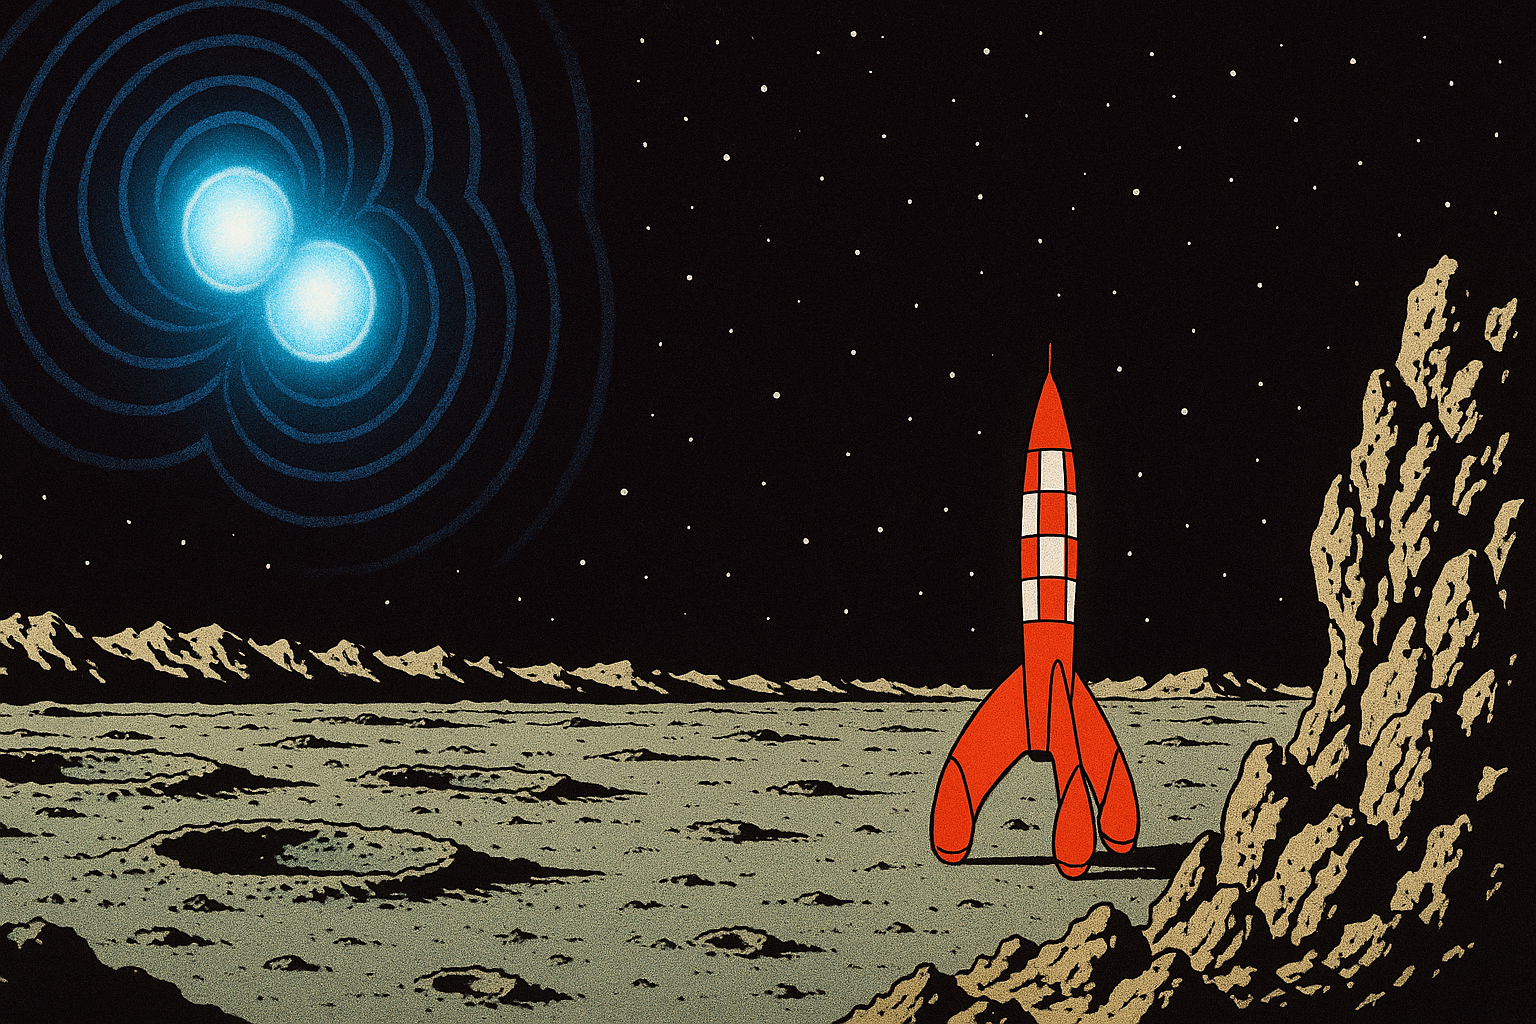
\includegraphics[width=\paperwidth,height=\paperheight]{Figures/tintin_BNS_2.png}}}

\begin{frame}[plain, noframenumbering]

  \begin{tikzpicture}[remember picture,overlay]
    \node[fill=customblue, fill opacity=0.75, text opacity=1, rounded corners=10pt, inner sep=15pt] at (current page.center) {
      \begin{minipage}{0.8\textwidth}
        \centering
        \textsc{jester}: \textsc{jax}-accelerated equation of state inference and TOV solvers \\[1.5ex]
        Thibeau Wouters \\[0.5ex]
        \github \quad \linkedin \quad \myemail
      \end{minipage}
    };
  \end{tikzpicture}

  \vspace{7cm}

  \begin{columns}
  \column{0.35\textwidth}
  \begin{figure}
    \centering
    \vspace{1.5mm}
    
\includegraphics[width=0.75\linewidth]{Figures/utrecht-university.png}
  \end{figure}
  \column{0.35\textwidth}
  \begin{figure}
    \centering
    
\includegraphics[width=0.75\linewidth]{Figures/Nikhef_logo-transparent.png}
  \end{figure}
\end{columns}

  \end{frame}
}


\begin{frame}[noframenumbering]
\frametitle{Table of Contents}
\tableofcontents[subsectionstyle=show/show/show]
\end{frame}

\section{Introduction}

\begin{frame}{Inverse problem of neutron stars}
  \def\x{2mm}

  \red{Inverse problem}: infer the EOS of dense nuclear matter from NS observations (masses, radii, tidal deformabilities, \dots)

  \vspace{\x}

  \begin{figure}
    \centering
    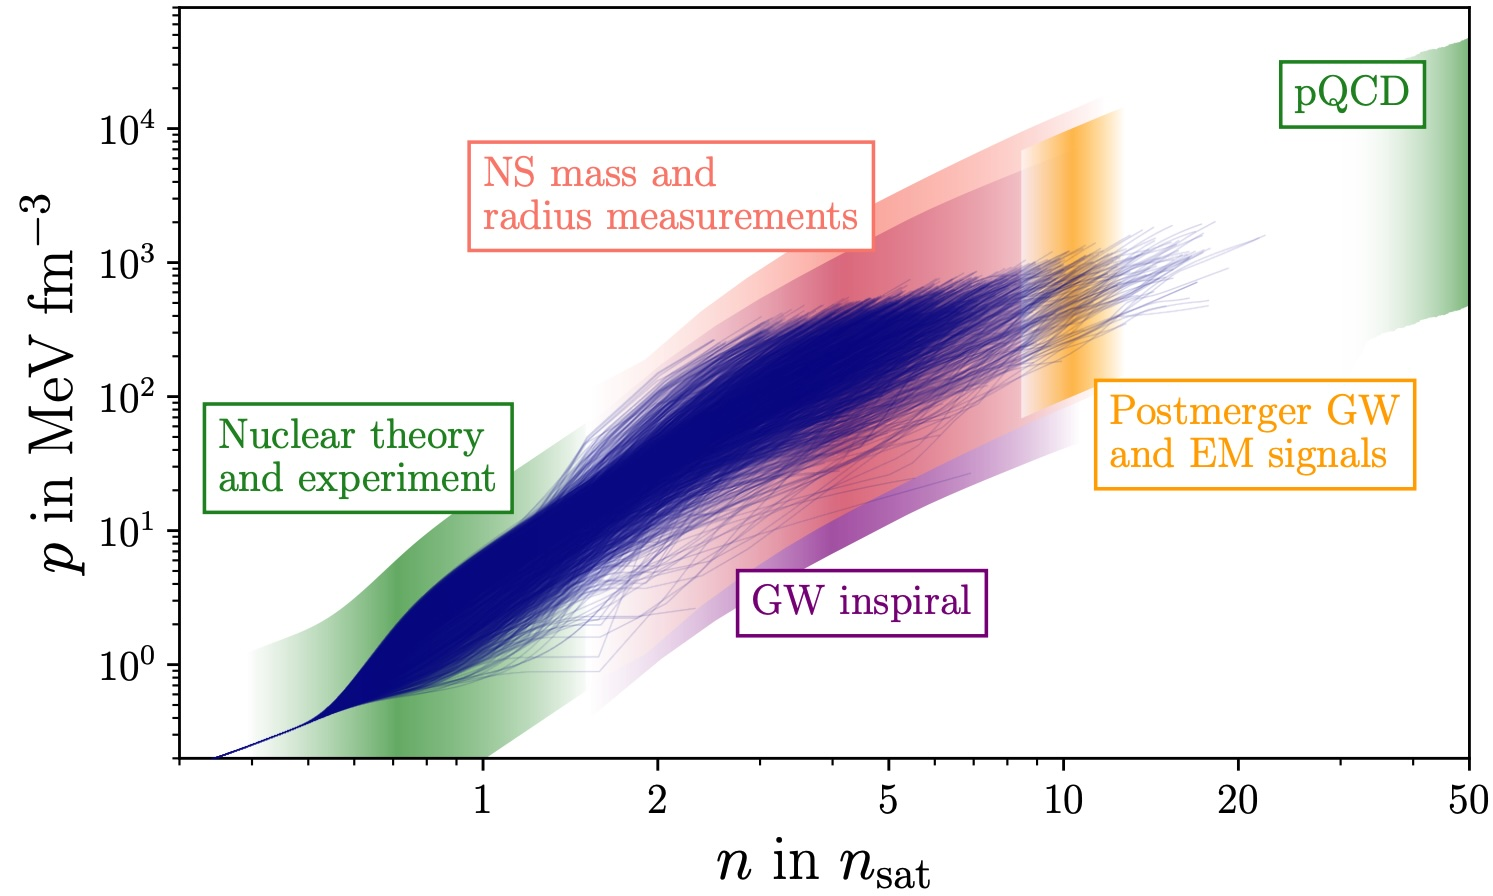
\includegraphics[width=0.80\linewidth]{Figures/Koehn_EOS.jpg}
  \end{figure}

\end{frame}


\begin{frame}{Parameter estimation: Bayesian inference}

  \def\x{5mm}

  How do we ``measure'' source parameters $\theta$ from data $d$?

  \vspace{\x}
  \pause

  Bayesian inference:
  \begin{equation*}
    p(\theta|d) = \frac{p(d|\theta)\, p(\theta)}{p(d)} = \frac{\rm{likelihood} \times \rm{prior}}{\rm{evidence}}
  \end{equation*}

  \vspace{\x}
  \pause

  Ingredients:
  \begin{itemize}
    \item Posterior: intractable, needs stochastic samplers
    \begin{itemize}
      \item MCMC, nested sampling, sequential Monte Carlo
    \end{itemize}

    \item Prior: encode beliefs about parameters

    \item Likelihood: \red{computational bottleneck}

    \item Evidence: model selection
  \end{itemize}
\end{frame}


\begin{frame}{Bayesian EOS inference}
  \def\x{4mm}
  \def\y{2mm}

  \begin{itemize}
    \item EOS constrained via Bayesian inference:
    \begin{equation*}
      p(\thetaeos | d) \propto \red{p(d | \thetaeos)} \, p(\thetaeos)
    \end{equation*}

    \vspace{\y}

    \item Sampling provides \blue{high number of effective samples}: direct, unbiased characterization of uncertainty
  \end{itemize}

  \vspace{\x}

  \centering
  \incfig[0.90\textwidth]{NS_likelihood}

\end{frame}


\begin{frame}{Computational bottleneck}
  \def\x{4mm}
  \def\y{2mm}

  \begin{itemize}
    \item Predict NS properties ($M$, $R$, $\Lambda$) from EOS: solve \red{TOV equations}

    \vspace{\x}

    \item $\mathcal{O}(10^5$--$10^6)$ likelihood calls per inference run

    \vspace{\x}

    \item \red{Bottleneck}: TOV solver speed determines total inference cost
  \end{itemize}

  \pause
  \vspace{\x}

  \begin{tcolorbox}[colback=blue!5!white,colframe=blue!75!black,title=Solution]
    GPU-accelerated, differentiable TOV solvers and samplers
  \end{tcolorbox}

\end{frame}

\section{What is \textsc{jester}?}

\begin{frame}{\textsc{jax}}

  \def\x{5mm}
  \def\y{1mm}

  \begin{columns}
    \begin{column}[t]{0.88\linewidth}
      \textsc{jax}~\ghlink{jax-ml/jax}~\cite{jax2018github}: \red{high-performance} numerical computing in Python
    \end{column}
    \begin{column}[t]{0.10\linewidth}
      \vspace{0pt}
      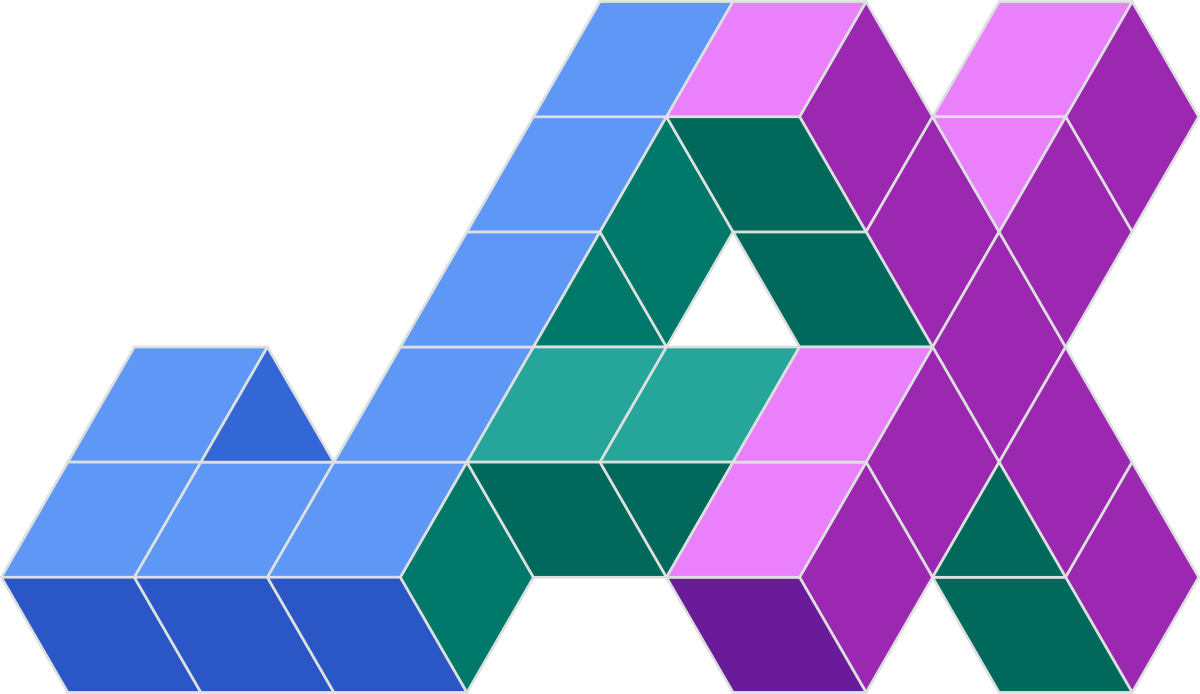
\includegraphics[width=0.85\linewidth]{Figures/jax.png}
    \end{column}
  \end{columns}

  \vspace{\x}
  \pause

  Gamechangers:
  \begin{itemize}
    \vspace{\y}
    \item Hardware accelerators: run Python on GPUs

    \vspace{\y}

    \item Composable function transformations:
    \begin{itemize}
      \item \jaxjit: just-in-time compilation
      \item \jaxgrad: automatic differentiation (exact, fast)
      \item \jaxvmap: vectorization / batch processing
    \end{itemize}
  \end{itemize}

  \pause
  \vspace{3mm}

  Example gradient descent on \textit{any} loss function:
  \begin{equation*}
    \boldtheta \leftarrow \boldtheta + \alpha\, \jaxvmap\!\left(\jaxjit(\jaxgrad(\mathcal{L}(\boldtheta)))\right)
  \end{equation*}

\end{frame}


\begin{frame}{\textsc{jester}: \textsc{jax}-accelerated EOS inference}
  \def\x{5mm}
  \def\y{1mm}

  \vspace{-4mm}

  \begin{columns}[t]
    \column{0.80\textwidth}
    \begin{itemize}
      \item Hierarchical EOS inference in JAX~\cite{Wouters:2025zju}
      \item GPU-accelerated TOV solvers and samplers
      \item \ghlink{nuclear-multimessenger-astronomy/jester}~\texttt{nuclear-multimessenger-astronomy/jester}
    \end{itemize}

    \column{0.20\textwidth}
    \begin{figure}
      \centering
      
\includegraphics[scale=0.05]{Figures/JESTER_logo.png}
    \end{figure}
  \end{columns}

  \vspace{\x}
  \pause

  Currently available:
  \begin{itemize}
    \vspace{\y}
    \item EOS models:
    \begin{itemize}
      \item Metamodel+speed-of-sound (MM+CSE)
      \item Spectral expansion
    \end{itemize}
    \vspace{\y}
    \item Samplers:
    \begin{itemize}
      \item \textsc{flowMC}~\cite{Gabrie:2021tlu,Wong:2022xvh}
      \item Nested sampling (NS)
      \item Sequential Monte Carlo (SMC)
    \end{itemize}
    \vspace{\y}
    \item Likelihoods: nuclear physics \& multimessenger data
  \end{itemize}
\end{frame}


\begin{frame}{EOS parametrization (1): metamodel}

  \def\x{3mm}

  \begin{itemize}
    \item At \red{low density}, we use the metamodel~\cite{Margueron:2017eqc,Margueron:2017lup}: Taylor expansion of energy per nucleon $E/A$ in\footnote{$n_{\rm{sat}} \equiv 0.16 \ \rm{fm}^{-3}$} $x = (n - n_{\rm{sat}}) / 3n_{\rm{sat}}$

    \vspace{\x}

    \item \red{Nuclear empirical parameters} (NEPs): coefficients of the expansion
  \end{itemize}

  \vspace{\x}

  \begin{equation*}
    E/A(n, \delta) = e_{\rm{sat}}(n) + e_{\rm{sym}}(n) \delta^2  + \mathcal{O}(\delta^4) \, , \quad \delta = (n_n - n_p) / n \,
  \end{equation*}

  \begin{align*}
    e_{\rm{sat}}(n) &= E_{\rm{sat}} + \tfrac12 K_{\rm{sat}} x^2 + \tfrac{1}{3!} Q_{\rm{sat}} x^3 + \tfrac{1}{4!} Z_{\rm{sat}} x^4 + \mathcal{O}(x^5) \\
    e_{\rm{sym}}(n) &= E_{\rm{sym}} + L_{\rm{sym}} x + \tfrac12 K_{\rm{sym}} x^2  \\
    & \quad + \tfrac{1}{3!} Q_{\rm{sym}} x^3 + \tfrac{1}{4!} Z_{\rm{sym}} x^4 + \mathcal{O}(x^5)
  \end{align*}

\end{frame}

\begin{frame}{EOS parametrization (2): high density}

  \def\x{3mm}
  \def\y{1mm}

  \begin{itemize}
    \item Metamodel breaks down at $\red{n_{\rm{break}}} \sim [1, 2] \ n_{\rm{sat}}$

    \vspace{\x}

    \item \red{Higher density}: parametrize the EOS with $c_s^2(n)$ grid points and linear interpolation~\cite{Somasundaram:2021clp}

    \vspace{\x}

    \item MM+CSE: $\gtrsim 25$ parameters $\thetaeos$ — \red{computationally challenging} for stochastic samplers (e.g.\ nested sampling)

  \end{itemize}

  \vspace{\y}

  \begin{figure}
    \centering
    
\includegraphics[width=0.60\linewidth]{Figures/cs2_sketch.pdf}
  \end{figure}
\end{frame}


\section{\textsc{jester} example}

\begin{frame}{Sequential Monte Carlo (SMC)}

  \def\x{4mm}
  \def\y{2mm}

  \begin{itemize}
    \item Compute posterior and Bayesian evidence

    \vspace{\y}

    \item Evolve swarm of particles through distributions~\cite{Williams:2025szm}:
    \begin{equation*}
      p_t(\theta | d) \propto p(d | \theta)^{\beta_t} p(\theta) \, , \quad \beta_t \in [0, 1] \, .
    \end{equation*}

    \vspace{\y}

    \item Parallelizable: efficient on GPU

    \vspace{\y}

    \item Well-suited for \blue{high-dimensional} parameter spaces
  \end{itemize}

  \begin{figure}
    \centering
    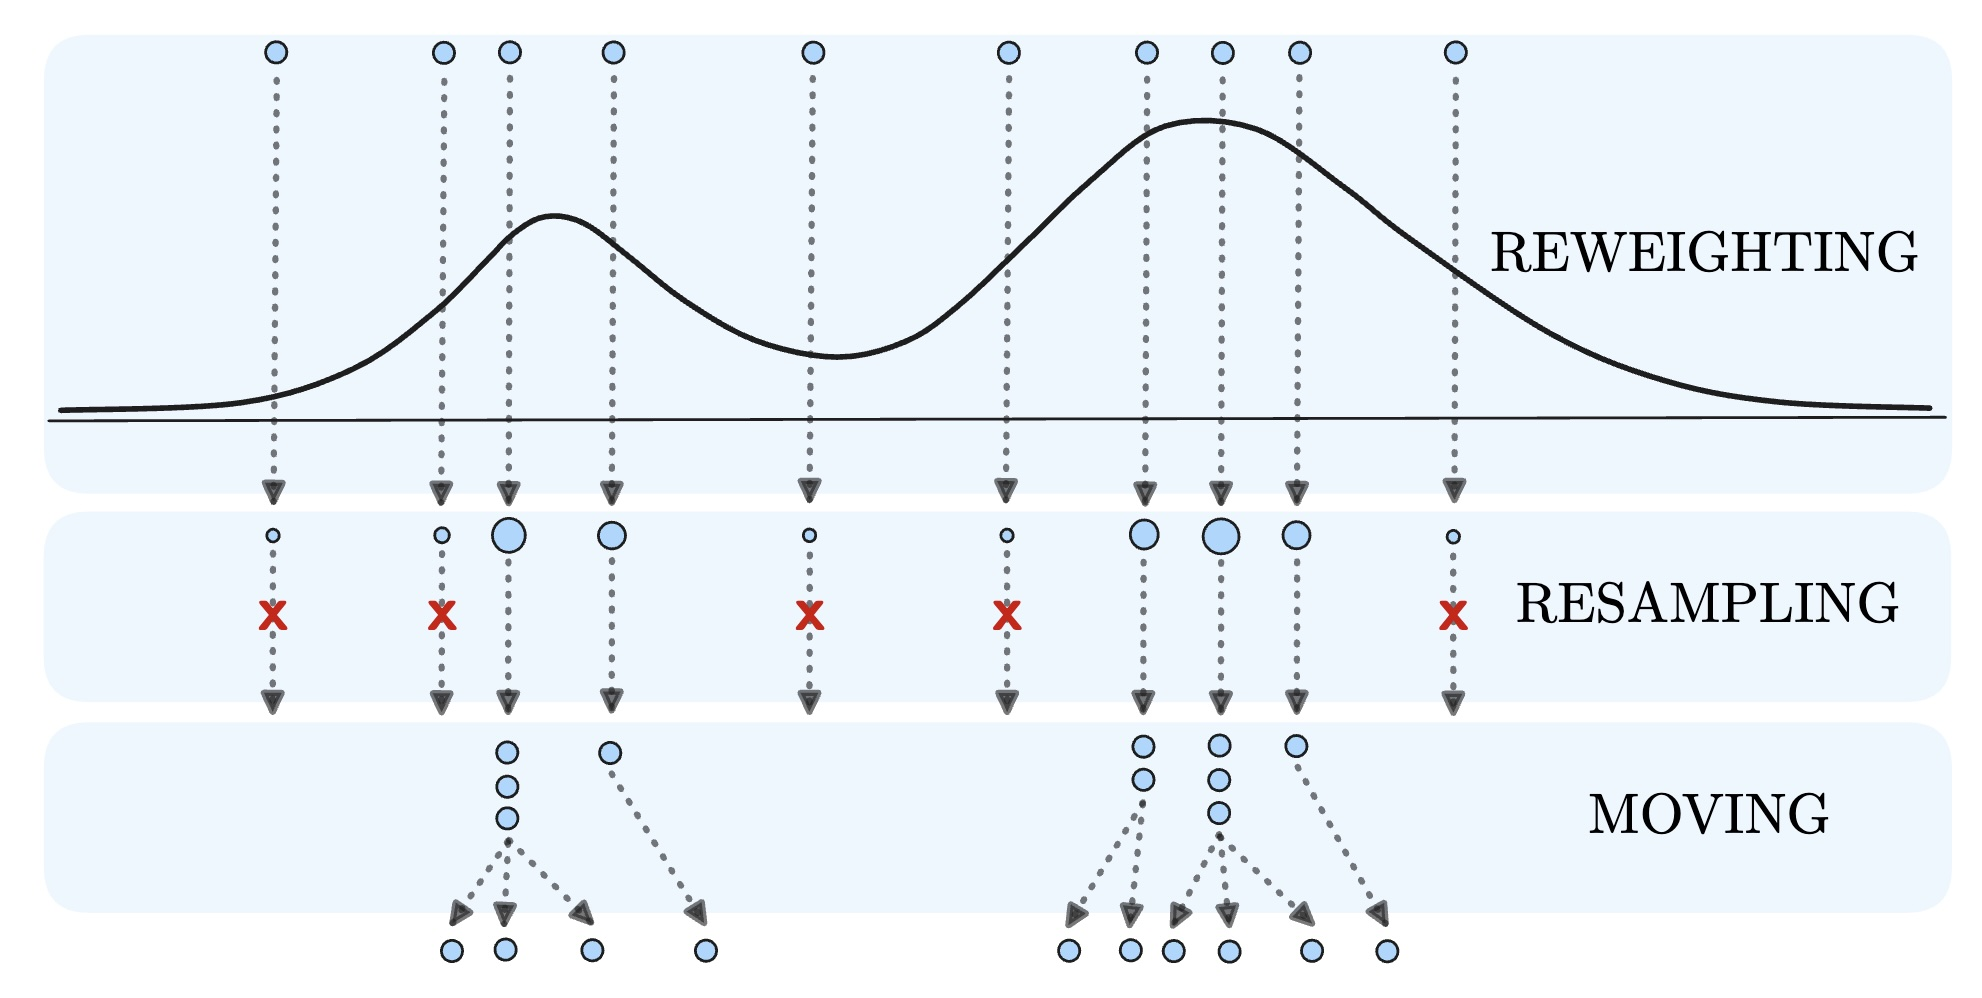
\includegraphics[width=0.70\textwidth]{Figures/SMC_diagram.jpg}
  \end{figure}
\end{frame}

\begin{frame}{Sampler systematics: GW170817}
  \def\x{4mm}
  \def\y{1mm}

  Analyzing GW170817 with different EOS and samplers — \blue{$\sim 5$ min per run} on H100 GPU:

  \vspace{-4mm}

  \begin{table}[h]
    \centering
    \renewcommand{\arraystretch}{1.4}
\begin{tabular}{p{4.5cm}cc}
    \hline
    EOS model & Sequential Monte Carlo & Nested Sampling \\
    \hline
    Metamodel\newline + speed-of-sound & $12.60^{+1.04}_{-1.42}$ & $12.46^{+1.15}_{-1.38}$ \\
    Spectral decomposition & $12.49^{+1.01}_{-1.33}$ & $12.40^{+1.03}_{-1.34}$ \\
    \hline
\end{tabular}

    \caption{$R_{1.4}$ [km] at 90\% credibility.}
  \end{table}

  \pause
  \vspace{-2mm}

  \begin{table}[h]
    \centering
    \renewcommand{\arraystretch}{1.4}
\begin{tabular}{p{4.5cm}cc}
    \hline
    EOS model & Sequential Monte Carlo & Nested Sampling \\
    \hline
    Metamodel\newline + speed-of-sound & 5m 38s & 32m 18s \\
    Spectral decomposition & 2m 57s & 7m 48s \\
    \hline
\end{tabular}

    \caption{Sampling time on 1 NVIDIA H100 GPU.}
  \end{table}
\end{frame}


\section{\textsc{jester} $\times$ CUTER}

\begin{frame}{Motivation}
  \def\x{5mm}
  \def\y{2mm}

  \begin{columns}[t]
    \column{0.48\textwidth}
    \textbf{CUTER} (nuclear physics):
    \begin{itemize}
      \vspace{\y}
      \item Microscopically motivated EOS models
      \vspace{\y}
      \item Nuclear theory constraints baked in
      \vspace{\y}
      \item \red{Missing}: fast Bayesian inference
    \end{itemize}

    \column{0.48\textwidth}
    \textbf{\textsc{jester}} (data analysis):
    \begin{itemize}
      \vspace{\y}
      \item GPU-accelerated samplers \& TOV solvers
      \vspace{\y}
      \item Flexible EOS models, but fixed crust
      \vspace{\y}
      \item \red{Missing}: richer nuclear physics
    \end{itemize}
  \end{columns}

  \vspace{\x}
  \pause

  \begin{tcolorbox}[colback=blue!5!white,colframe=blue!75!black,title=Goal]
    Connect both sides: fast Bayesian inference of microscopically motivated EOS models with \textsc{jester} + CUTER
  \end{tcolorbox}

\end{frame}

\begin{frame}{\textsc{jester} $\times$ CUTER}
  \def\x{3mm}
  \def\y{1mm}

  Ongoing developments in \textsc{jester}-land:
  \begin{itemize}
    \vspace{\y}
    \item Documentation and examples: welcome to start using \textsc{jester}!
    \vspace{\y}
    \item Scalar-tensor TOV solver, NS anistropy,\dots projection studies for ET
    \vspace{\y}
    \item dUrca process (Guilherme Grams)
    \vspace{\y}
    \item GW+EM constraints, EOS+population inference (Hauke Koehn)
    \vspace{\y}
    \item Weekly meetings: Monday at 15:00 CET (but flexible)
  \end{itemize}

  Other ideas for connecting \textsc{jester} and CUTER:
  \begin{itemize}
    \vspace{\y}
    \item Fixed crust $\rightarrow$ consistent crust (CUTER translated to JAX?)
    \vspace{\y}
    \item New metamodel EOS in \textsc{jester} (Gabriele's work)
    \vspace{\y}
    \item Waveform systematics (Adrian)
    \vspace{\y}
    \item Finite temperature, composition
    \vspace{\y}
    \item \dots
  \end{itemize}

\end{frame}


\section{Applications}

\subsection{ET projections}

\begin{frame}{Future observing runs}
  \def\x{6mm}
  \def\y{2mm}

  \begin{itemize}
    \item Sampling systematics under control for GW170817

    \vspace{\y}

    \item But... what about future observing runs?
  \end{itemize}

  \pause
  \vspace{\x}

  Simulated study for Einstein Telescope (ET):
  \begin{itemize}
    \vspace{\y}
    \item 100 loudest BNS events from 1 year (CoBa catalogue~\cite{Branchesi:2023mws})

    \vspace{\y}

    \item GW parameter estimation
    \begin{itemize}
      \item \textsc{IMRPhenomXP\_NRTidalv3}, $f_{\rm{min}} = 5$ Hz
      \item Relative binning
      \item Done by Fabian Gittins
    \end{itemize}

    \vspace{\y}

    \item \red{Preliminary results!}

  \end{itemize}
\end{frame}

\begin{frame}{ET projections: Results}
  \def\x{7mm}
  \def\y{2mm}

  \vspace{\x}

  \only<1>{
    \begin{figure}
    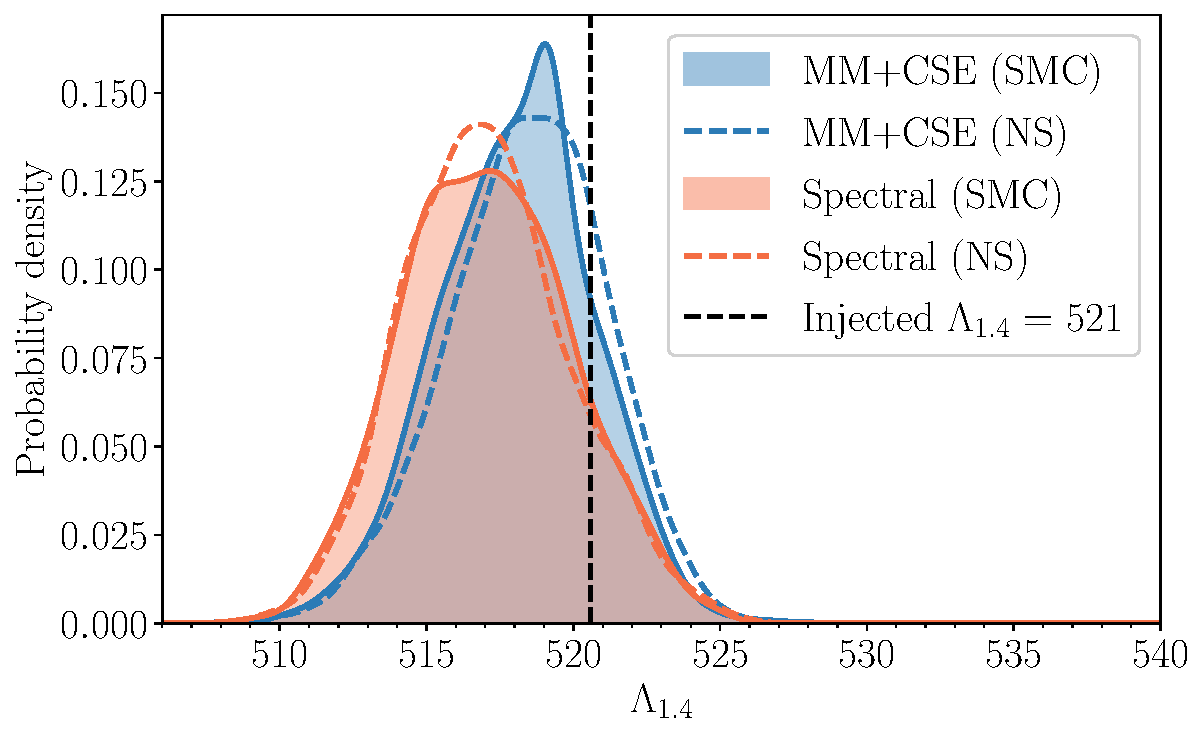
\includegraphics[width=0.90\textwidth]{ET_ET_lambda14_comparison.pdf}
    \end{figure}
  }

  \only<2>{
    \begin{figure}
    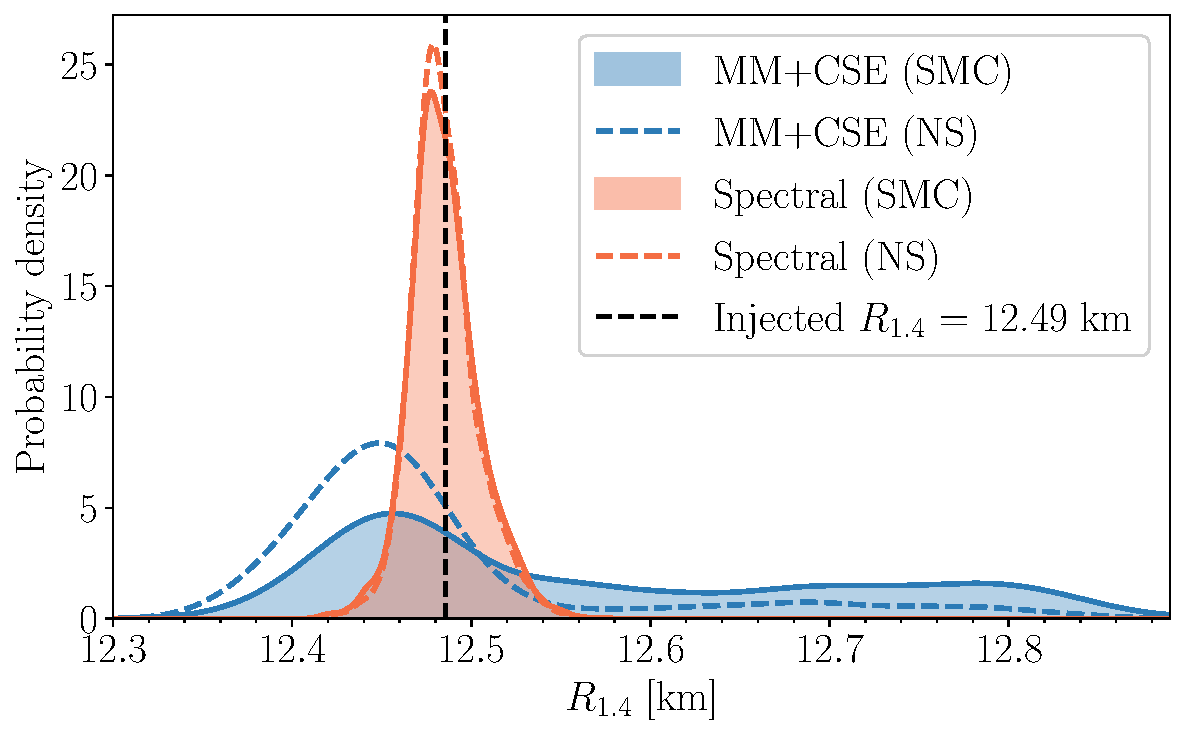
\includegraphics[width=0.90\textwidth]{ET_ET_r14_comparison.pdf}
    \end{figure}
  }

  \only<3>{
    \vspace{-3mm}
    \begin{figure}
    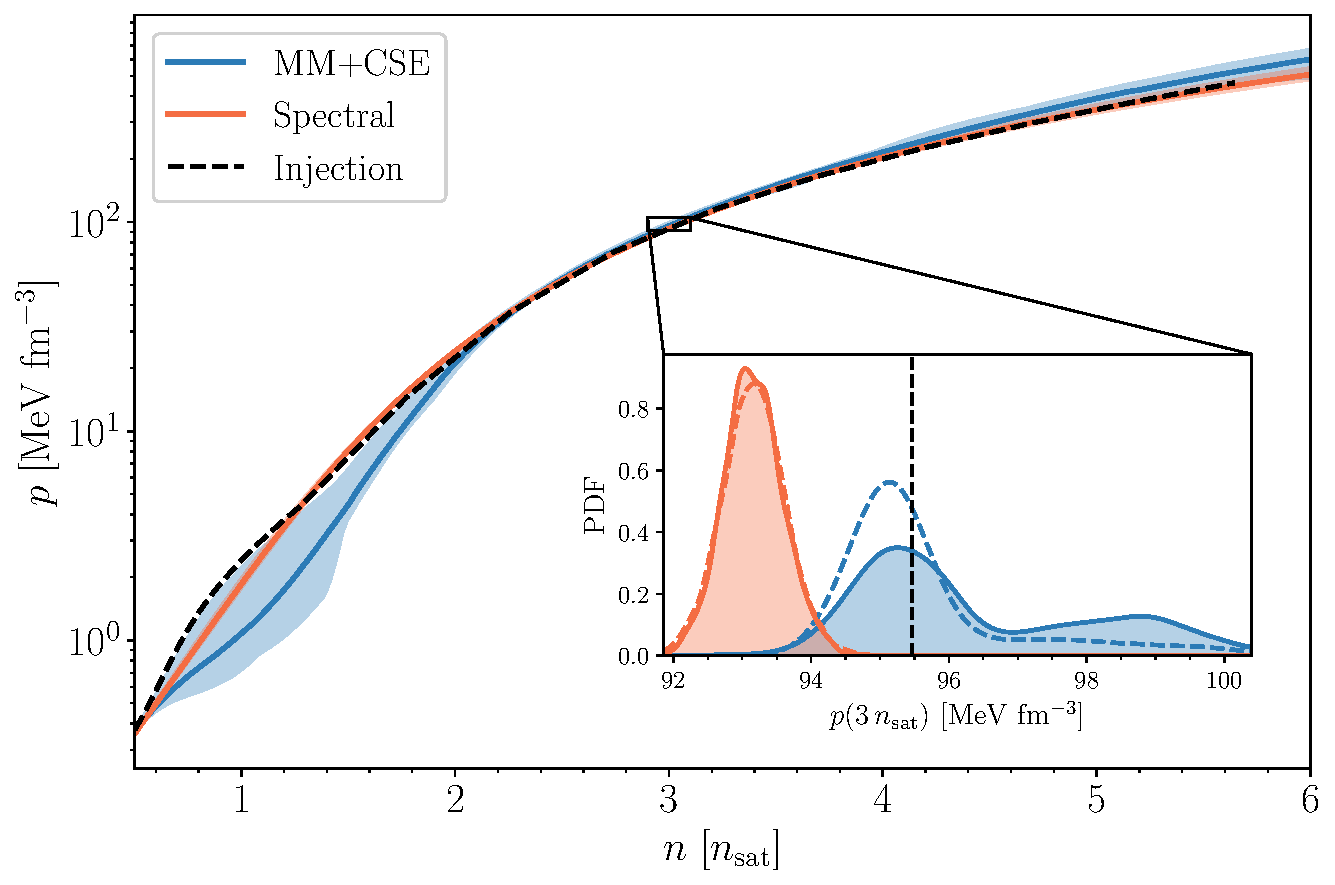
\includegraphics[width=0.90\textwidth]{Figures/ET_pressure_density_inset.pdf}
    \end{figure}
  }

\end{frame}

\begin{frame}{ET projections: Summary}
  \def\x{3mm}
  \def\y{2mm}

  \vspace{-4mm}

  \begin{table}[h]
    \centering
    \renewcommand{\arraystretch}{1.4}
\begin{tabular}{p{4.5cm}cc}
    \hline
    EOS model & Sequential Monte Carlo & Nested Sampling \\
    \hline
    Metamodel\newline + speed-of-sound & $12.51^{+0.31}_{-0.10}$ & $12.45^{+0.29}_{-0.07}$ \\
    Spectral decomposition & $12.48^{+0.04}_{-0.03}$ & $12.48^{+0.04}_{-0.02}$ \\
    \hline
\end{tabular}

    \caption{$R_{1.4}$ [km] at 90\% credibility.}
  \end{table}

  \vspace{-4mm}
  \pause

  \begin{table}[h]
    \centering
    \renewcommand{\arraystretch}{1.4}
\begin{tabular}{p{4.5cm}cc}
    \hline
    EOS model & Sequential Monte Carlo & Nested Sampling \\
    \hline
    Metamodel\newline + speed-of-sound & 1h 24m & 13h 07m \\
    Spectral decomposition & 20m 10s & 1h 11m \\
    \hline
\end{tabular}

    \caption{Sampling time on 1 NVIDIA H100 GPU.}
  \end{table}

\end{frame}


\subsection{Pressure anisotropy}

\begin{frame}{Pressure anisotropy in neutron stars}

  \def\x{3mm}
  \def\y{1mm}

  \vspace{-3mm}

  \begin{columns}
    \begin{column}{0.55\textwidth}
      \begin{itemize}
        \item Standard TOV: assumes \blue{isotropic pressure} ($p_r = p_t$)

        \vspace{\x}

        \item Physical mechanisms can violate this (pion/kaon condensation, magnetic fields, superfluidity)

        \vspace{\x}

        \item Anisotropy parameter $\sigma \equiv p_r - p_t$; model:
        \begin{equation*}
          \sigma = \red{\gamma} \,\frac{2m p_r}{r}
        \end{equation*}
      \end{itemize}
    \end{column}
    \begin{column}{0.44\textwidth}
      \begin{figure}
        \centering
        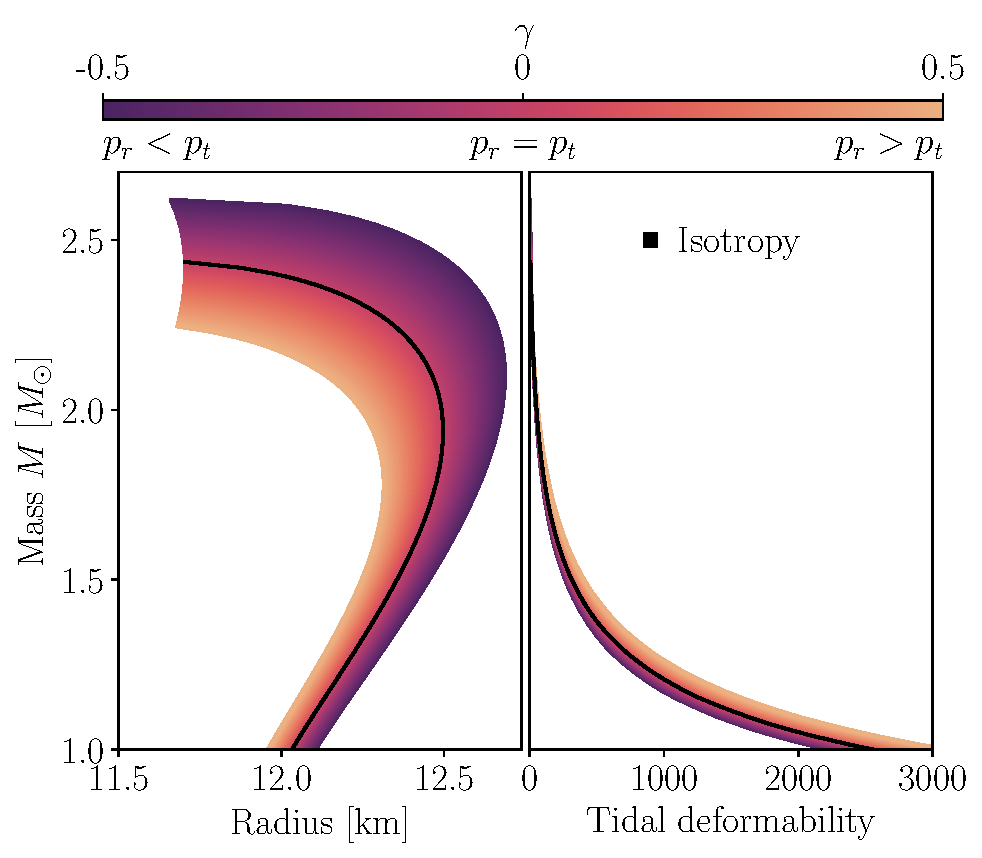
\includegraphics[width=0.99\linewidth]{Figures/pressure_anistropy_demo_art.pdf}
      \end{figure}
    \end{column}
  \end{columns}

  \vspace{\x}

  \begin{tcolorbox}[colback=blue!5!white, colframe=blue!75!black]
    Key question: can we ``measure'' anisotropy ($\gamma \neq 0$) with current data?
  \end{tcolorbox}

\end{frame}


\begin{frame}{Measuring anisotropy with \textsc{jester}}

  \def\x{3mm}
  \def\y{1mm}

  Modified TOV equations with anisotropic pressure~\cite{Pang:2025fes}:
  \begin{itemize}
    \vspace{\y}
    \item $\gamma$ enters the structure equations and tidal deformability
    \vspace{\y}
    \item Implemented as additional free parameter in \textsc{jester}
  \end{itemize}

  \pause
  \vspace{\x}

  Hierarchical Bayesian inference across multiple neutron stars:
  \begin{itemize}
    \vspace{\y}
    \item Multimessenger data: GW + NICER + nuclear theory
    \vspace{\y}
    \item $\gamma$ allowed to vary \emph{per star} (breaks EOS degeneracy)
    \vspace{\y}
    \item Model selection: anisotropic vs isotropic hypothesis
  \end{itemize}

\end{frame}


\begin{frame}{Anisotropy results~\smallcite{Pang:2025fes}}

  \def\x{3.5mm}

  \begin{columns}
    \begin{column}{0.58\textwidth}
      \begin{figure}
        \centering
        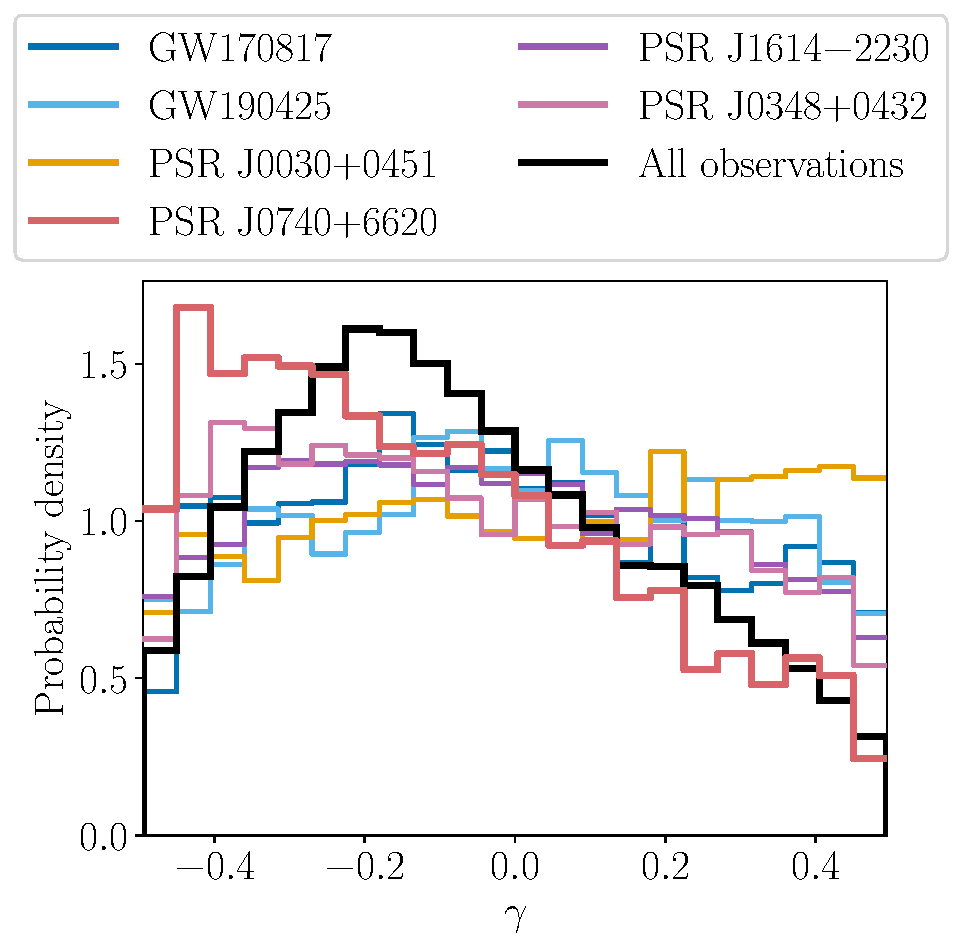
\includegraphics[width=0.99\linewidth]{Figures/individual_gamma_hist_noGaussian.pdf}
      \end{figure}
    \end{column}

    \begin{column}{0.41\textwidth}
      \begin{itemize}
        \item Preference for \red{negative} anisotropy

        \vspace{\x}

        \item Driven by \red{PSR J0740+6620} (NICER)

        \vspace{\x}

        \item Bayes factor $\gtrsim 3:1$ for anisotropy vs isotropy

        \vspace{\x}

        \item Evidence inconclusive, but anisotropy remains a useful probe
      \end{itemize}
    \end{column}
  \end{columns}

\end{frame}


\subsection{Gradient-based optimization}

\begin{frame}{Gradient-based optimization}

  \def\x{2mm}

  \begin{itemize}
    \item Given $\hat{R}(M)$ or $\hat{\Lambda}(M)$: recover EOS parameters $\thetaeos$

    \vspace{\x}

    \item Loss function $L(\thetaeos)$: relative error in tidal deformability $\Lambda$

    \vspace{\x}

    \item Gradient descent: $\boldtheta^{(i+1)} \leftarrow \boldtheta^{(i)} - \gamma \nabla L(\boldtheta^{(i)})$ with Adam
    \begin{itemize}
      \item Automatic differentiation!
    \end{itemize}

  \end{itemize}

  \vspace{-3mm}

  \begin{columns}

    \column{0.45\textwidth}

    \small
    \begin{equation*}
      L(\thetaeos) = \frac1N \sum_{i=1}^N \left| \frac{\Lambda_i(\thetaeos) - \hat{\Lambda}_i}{\hat{\Lambda}_i} \right|
    \end{equation*}

    \normalsize

    \column{0.60\textwidth}

    \begin{figure}[htpb]
      \centering
      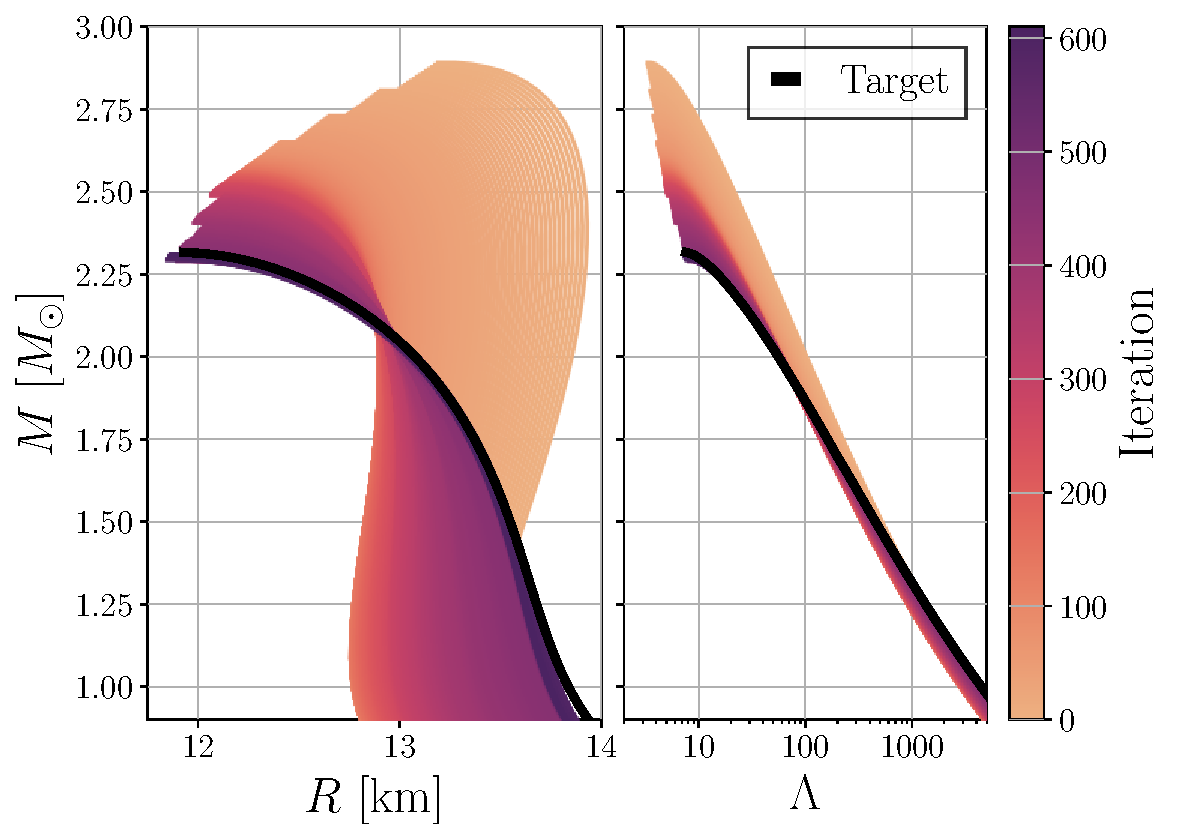
\includegraphics[width=1.0\linewidth]{Figures/showcase_variational_inference.pdf}
    \end{figure}

  \end{columns}
\end{frame}

\begin{frame}{Recovery of nuclear empirical parameters}

  \def\x{3mm}
  \def\y{2mm}

  What do NSs tell us about nuclear empirical parameters (NEPs)?

  \vspace{\y}

  \begin{itemize}
    \item Use only NEPs -- no $c_s^2(n)$ grid points

    \vspace{\x}

    \item If more NEPs are varied, $L_{\rm{sym}}$ is no longer constrained

    \vspace{\x}

    \item Recovered EOSs deviate $<100$ meters, $<10$ in $\Lambda$ from the true EOS
  \end{itemize}

  \begin{figure}
    \centering
    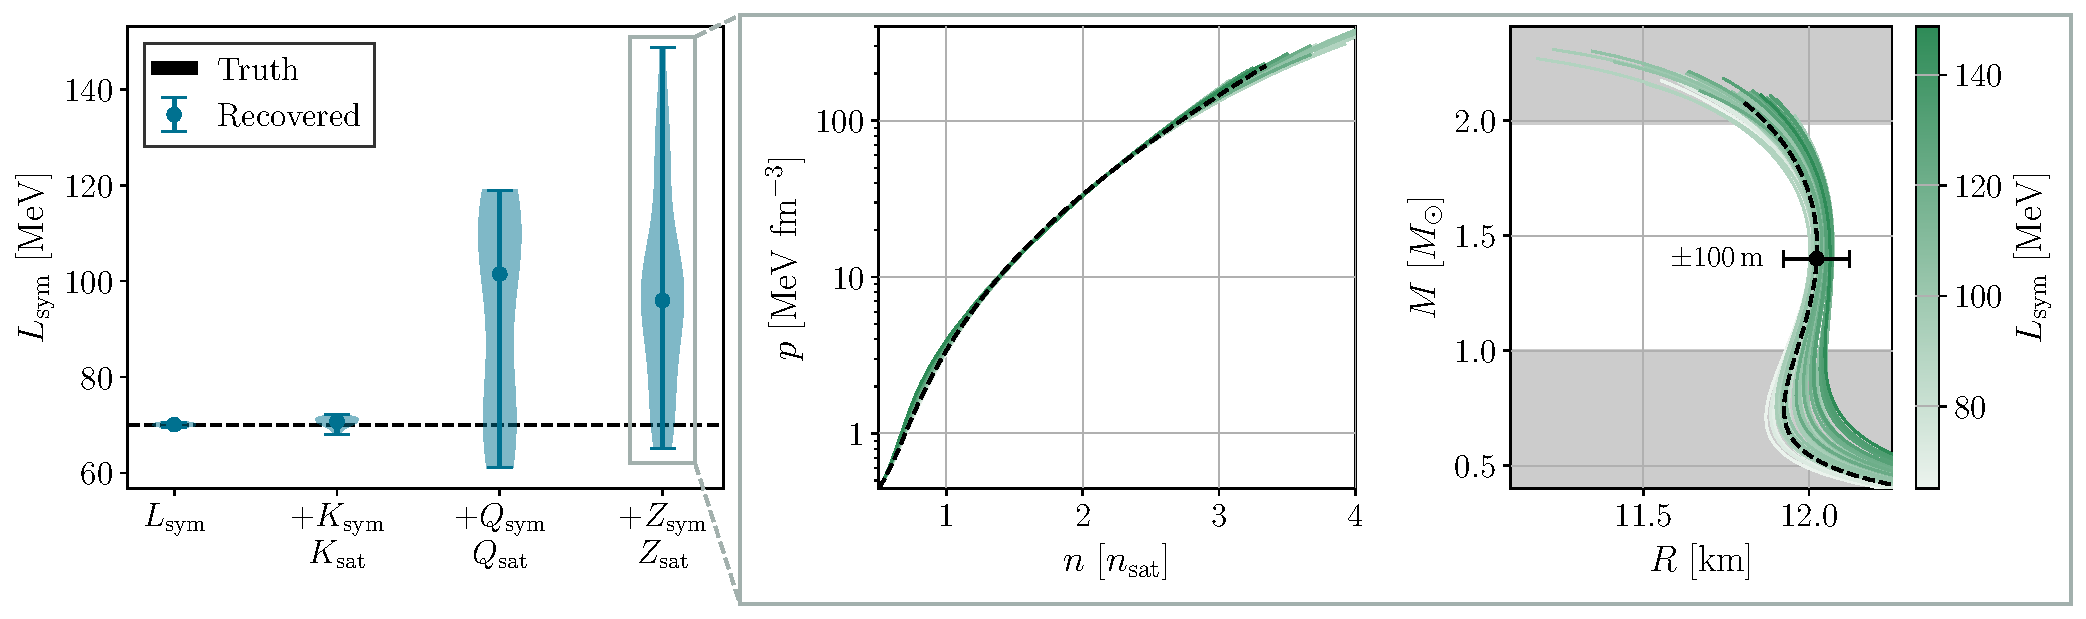
\includegraphics[width=1.0\linewidth]{Figures/money_plot.pdf}
  \end{figure}
\end{frame}


\section{Outlook \& Conclusion}

\begin{frame}{Conclusion}
  \def\x{4mm}

  \begin{itemize}
    \item \textsc{jester}: GPU-accelerated, differentiable EOS inference framework

    \vspace{\x}

    \item Bayesian inference: scalable, $\sim 1$ h on H100 for GW170817

    \vspace{\x}

    \item Gradient-based optimization: recover NEPs from NS observables

    \vspace{\x}

    \item Sampler systematics under control; ET projections in progress

    \vspace{\x}

    \item \blue{CUTER + jester}: nuclear physics meets scalable inference
  \end{itemize}

\end{frame}

{
\usebackgroundtemplate{\transparent{0.5}{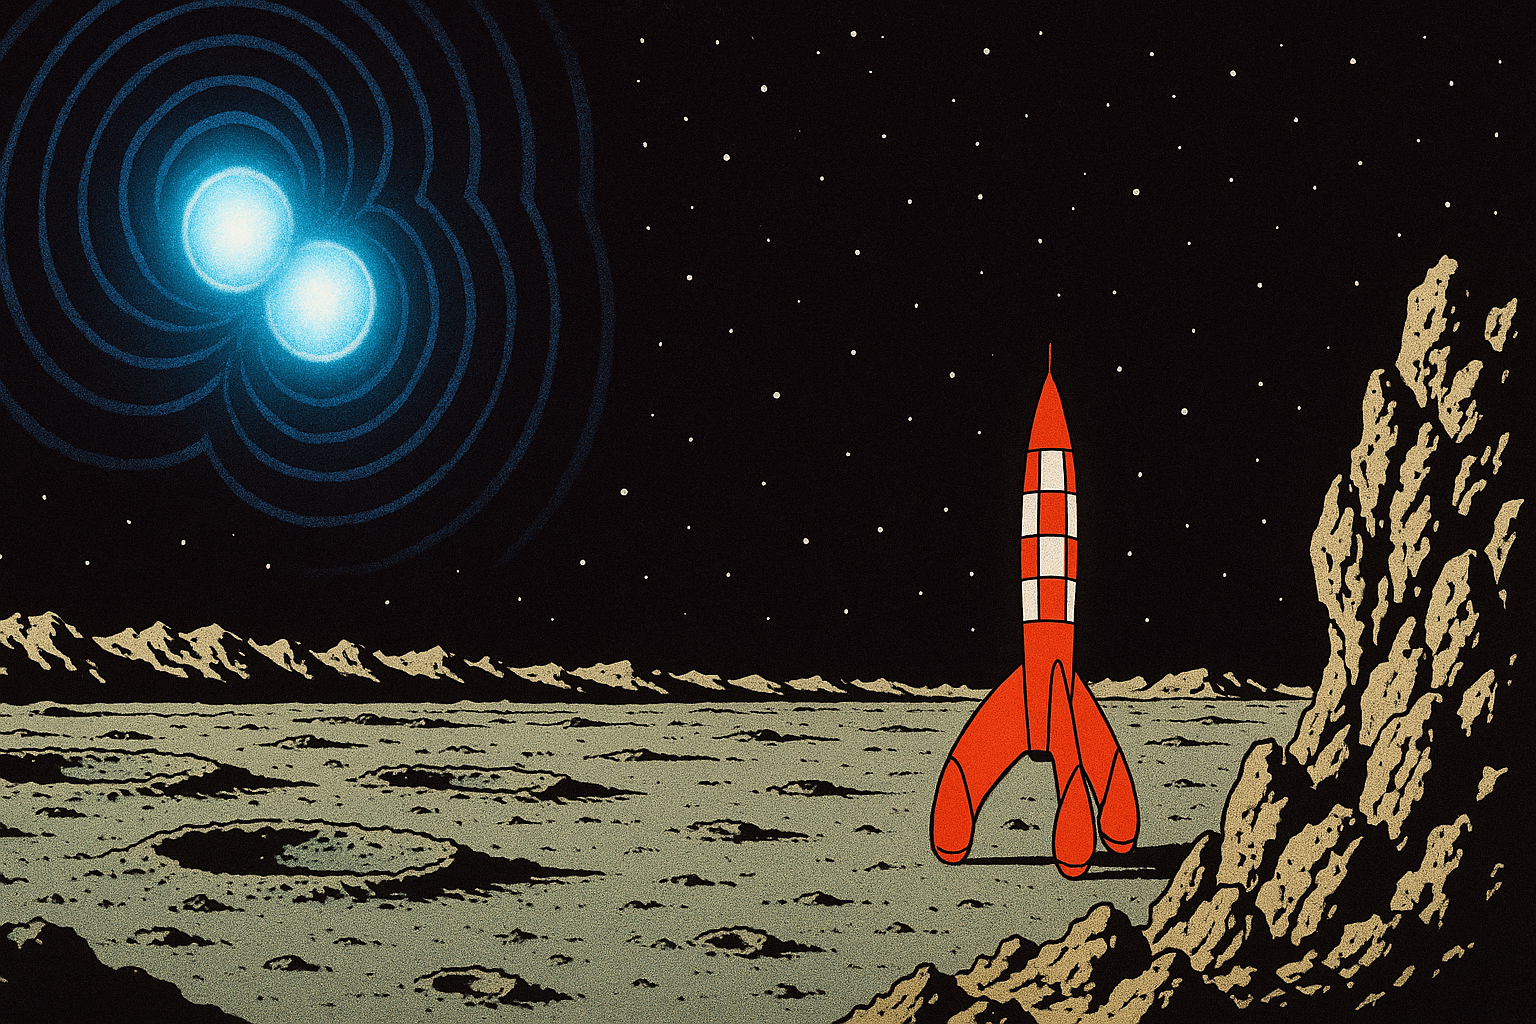
\includegraphics[width=\paperwidth,height=\paperheight]{Figures/tintin_BNS_2.png}}}

\begin{frame}[plain, noframenumbering]

  \begin{tikzpicture}[remember picture,overlay]
    \node[fill=customblue, fill opacity=0.75, text opacity=1, rounded corners=10pt, inner sep=15pt] at ([yshift=2cm]current page.center) {
      \begin{minipage}{0.8\textwidth}
        \centering
        \textbf{Thanks for listening!}
      \end{minipage}
    };
  \end{tikzpicture}

  \end{frame}
}

\begin{frame}[allowframebreaks]{References}
  \printbibliography
\end{frame}

\end{document}
